% !TEX root = ../../semexp-thesis.tex

\section{Architecture}
\label{sec:design/architecture}

\begin{figure}
	\centering
	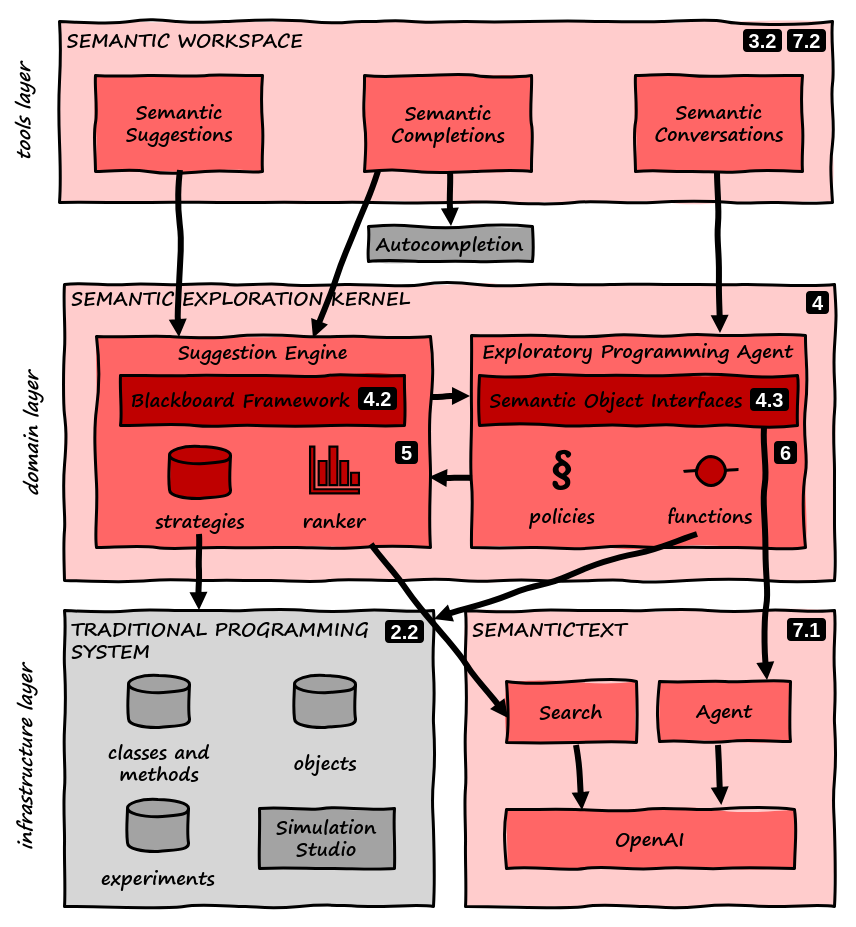
\includegraphics[width=\textwidth]{01_architecture/architecture.png}
	\caption[The high-level architecture of the \emph{semantic exploration kernel} and its environment.]{
		The high-level architecture of the \emph{semantic exploration kernel} and its environment.
		The architecture is structured in three layers for semantic tools, domain concepts, and underlying infrastructure.

		\capparagraph{Legend.}
		New components are \bold{\gradientHSB{colorful}{-45,240,200}{195,240,200}} and existing components are \bold{\textcolor{gray}{gray}}.
		Arrows indicate dependencies from a higher-level component to a lower-level component.
		\CircledInverted{Numbers} reference the chapter, section, or appendix in this thesis that further describes a component.
	}
	\label{fig:design/architecture/architecture}
\end{figure}

\Cref{fig:design/architecture/architecture} displays the high-level architecture of the semantic exploration kernel and its environment.
The overarching semantic exploratory programming system can be divided into three layers: the \emph{semantic workspace} for (graphical) programming tooling, the \emph{semantic exploration kernel} for the domain logic of the system, and the \emph{infrastructure layer} for required packages and integrations.

The semantic workspace provides different semantic tools, through which programmers can interact with the system~(\cref{sec:approach/workspace}).
The semantic exploration kernel consists of two components for processing the semantic context of the programming session and augmenting it: the suggestion engine and the exploratory programming agent.

\begin{description}[noextralabelsep]
	\item[The suggestion engine] captures the implicit concept of programmers from their previous experiments, reconstructs their plans and intentions, and creates new suggestions.
	For this, it defines a \emph{blackboard framework}, which manages various \emph{artifacts} such as methods, classes, and scripts and orchestrates \emph{strategies} for suggesting new artifacts based on existing ones~(\cref{sec:design/suggestions}).
	Next to the generic framework, the suggestion engine also provides several types of artifacts and strategies that employ semantic retrieval methods for searching objects, generating experiments, and structuring and ranking results~(\cref{cha:suggestions}).
	\item[The exploratory programming agent] receives explicit questions and answers them by autonomously conducting exploratory research processes.
	It connects to its environment through \emph{semantic object interfaces}, which allow programmers to ask semantic questions to objects in the system~(\cref{sec:design/agent}).
	Internally, it employs a generative LLM to support natural-language conversations and machine reasoning.
	The agent is configured through a set of \emph{policies}, which define its behavior, and a set of \emph{system functions}, through which the agent can interact with objects in the system~(\cref{cha:agent}).
\end{description}

The suggestion engine and the exploratory programming agent can interact with each other:
particular strategies that require reasoning about other artifacts or code generation invoke the exploratory programming agent.
In the other direction, when the agent needs a broader overview of system parts, it will employ the suggestion engine to retrieve relevant artifacts.

Both the semantic workspace and the semantic exploration kernel require a traditional exploratory programming system~(\cref{cha:implementation}).
The semantic workspace integrates semantic interfaces for its tools into the existing programming system, for example, through a completion menu in code editors or a conversational interface in several exploration tools.
Similarly, it also hooks into the existing user interface to observe experiments through artifacts such as opened tabs and windows.
The exploration kernel interacts with the traditional system to access classes, methods, and objects for retrieving suggestions or executing experiments.

In our implementation, the semantic workspace and the exploration kernel also depend on a couple of other packages:

\begin{description}
	\item[\semtex:]
	The exploration kernel uses our \semtex framework\footnote{\url{https://github.com/hpi-swa-lab/Squeak-SemanticText}}, which provides access to semantic technologies for retrieving documents, generating text with conversational LLMs, and implementing specialized agents~(\cref{apx:semtex}).
	This framework also provides a graphical user interface component for conversational agents, which is employed by the semantic workspace for semantic conversations.

	\item[\simstudio:]
	Furthermore, the exploration kernel uses our \simstudio framework for instrumented code interpretation\footnote{\url{https://github.com/LinqLover/SimulationStudio}} to construct a dynamic call graph about suggested methods (\emph{method harvesting}, \cpageref{sec:suggestions/search/correlations}) and execute experiments from the agent in an isolated sandbox~(\cref{sec:agent/interfaces}).

	\item[\name{Autocompletion}:]
	Finally, we use and extend the \name{Autocompletion} package\footnote{\url{https://github.com/LeonMatthes/Autocompletion}} to integrate semantic completions into the programming system~(\cref{sec:implementation/completions}).
\end{description}

In the following sections, we introduce our blackboard framework for the suggestion engine and semantic object interfaces for the exploratory programming agent.
